\section{Improved Method (v2)}
\label{sec:v2}

We propose two structural changes. Both are zero-parameter --- they shape \emph{how} existing weights are used, not how many there are.

\subsection{Fix 1: gate floor reparameterization}

Replace the plain sigmoid with
\begin{equation}
    g_{\mathrm{eff}} \;=\; \mathrm{floor} + (1 - \mathrm{floor}) \cdot \sigma(\alpha), \qquad \mathrm{floor} \in [0, 1).
    \label{eq:gate-floor}
\end{equation}
With $\mathrm{floor} = 0.1$ and $\alpha_{\mathrm{init}} = 0$, the effective gate begins at $0.55$ and is bounded below by $0.1$ regardless of optimizer pressure. Figure~\ref{fig:gate-reparam} shows the curve.

\begin{figure}[H]
    \centering
    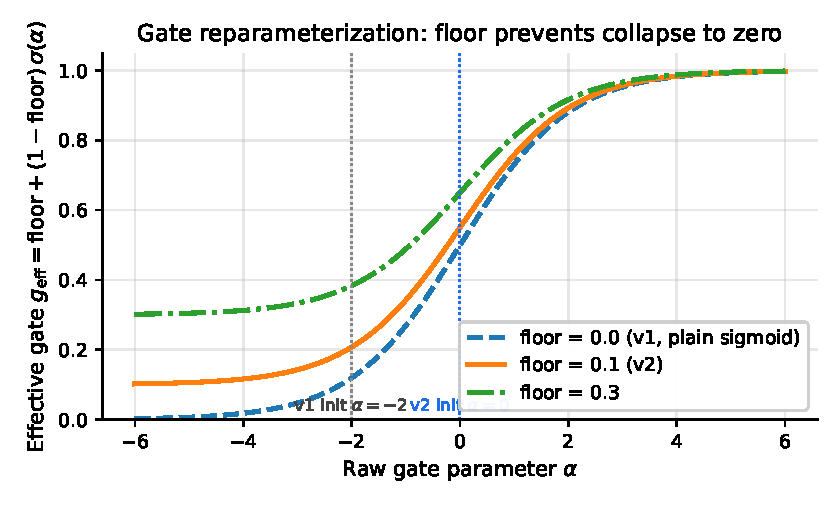
\includegraphics[width=0.65\textwidth]{figures/gate_reparam.pdf}
    \caption{Gate reparameterization. The plain sigmoid (dashed) saturates to zero on its left tail; v1's $\alpha=-2$ initialization sits in that saturating region. The floored variant (solid) is bounded below at $0.1$, leaving the optimizer free to attenuate the feedback but unable to silence it.}
    \label{fig:gate-reparam}
\end{figure}

\noindent\textbf{Why it works.} The reparameterization removes a degree of freedom the optimizer does not need: the option of driving the gate to zero. The model can still learn to attenuate the feedback contribution if attenuation reduces the loss, but the floor guarantees the cross-attention output always has a non-trivial weight when added back to memory. The mechanism is structurally guaranteed to remain in the loop at training and at inference.

\subsection{Fix 2: level mask}

We restrict the cross-attention in Equation~\ref{eq:feedback} to a subset of pyramid levels. Concretely, given a Boolean mask $\mathbf{b} \in \{0, 1\}^{4}$ over (P2, P3, P4, P5), the feedback is computed only on the union of token positions corresponding to active levels, and only those positions are written back. Inactive level positions in $\mathbf{m}$ pass through byte-identical.

We use $\mathbf{b} = (1, 1, 0, 0)$: refine P2 (stride 4) and P3 (stride 8), leave P4 and P5 untouched.

\noindent\textbf{Why it works.} Small objects live in stride-4 and stride-8 features. A single cross-attention pattern cannot simultaneously be optimal for sub-pixel-precise stride-4 tokens and for stride-32 tokens that each cover a large neighborhood; v1 forced the same mechanism to do both, and the gradient signal got diluted. The mask focuses the refinement on the levels that carry small-object signal, which is the metric we want to move. As a side effect, it also reduces compute (the cross-attention runs on a memory subset).

\subsection{What v2 does \emph{not} change}

Same architecture, same parameter count (49.08\,M), same training pipeline, same hyperparameters, same loss. The only differences from v1 are Equation~\ref{eq:gate-floor} and the level mask. Everything else is held fixed --- which is what makes the result in Section~\ref{sec:ablation} attributable to these two changes.
